\documentclass[11pt, class=article, crop=false]{standalone}
\usepackage[subpreambles=true]{standalone}
\usepackage[T1]{fontenc} % for font setting
\usepackage{newtxtext,newtxmath}
\usepackage{import,
            graphicx,
            parskip,
            url,
            amsmath,
            wrapfig,
            fancyhdr,
            soul,
            tabularx,
            authblk,
            textcomp,
            lineno}

% side caption figure
\usepackage{sidecap}
\sidecaptionvpos{figure}{t}

% for special characters in bibliography            
\usepackage[utf8]{inputenc}
\usepackage[T1]{fontenc}

% citation setup
\usepackage[euler]{textgreek}
\usepackage[sort&compress]{natbib}
\usepackage[utf8]{inputenc}
\setcitestyle{square}
\setcitestyle{comma}
\bibliographystyle{vancouver} % for prceedings B (Royal society publishing)

% caption setup
\usepackage[font = small, labelfont = {bf, small}]{caption}
           
% margin
\usepackage[top=2.54cm, bottom=2.54cm, left=2.54cm, right=2.54cm]{geometry}

% title
\title{Body size and local density explain movement patterns in stream fish}
\date{} % remove date from title

% author list
\author{} % remove author list from main text

\linenumbers

\begin{document}

\maketitle

\section{Abstract}

Movement is a fundamental process in structuring communities and distributing species. Both extrinsic (e.g., density of species) and intrinsic factors (e.g., body size) influence movement patterns, ultimately driving the spatial organization of communities. However, these extrinsic and intrinsic factors are often assessed in isolation, limiting our ability to understand how multiple factors combine to shape movement patterns in nature. Here, we evaluate whether body size and intra- and interspecific densities have an impact on movement of four fish species: bluehead chub, creek chub, green sunfish, and redbreast sunfish in a small stream. We applied a dispersal-observation model accounting for detectability, survival, and emigration to capture-mark-recapture data to estimate movement patterns. We found that larger individuals were more likely to move, which may be explained by their greater physical ability to balance the energetic cost of moving in tandem with heightened competitive ability during settlement. The effect of density on movement was mixed, such that both centrarchid species responded positively to creek chub, but conversely to the bluehead chub. However, cyprinid responses were limited and variable. These results suggest drivers of movement are species-specific, but further integration of behavioral and spatial ecology can provide greater insight into spatial dynamics. 

\section{Introduction}

Local communities are dynamically linked to each other via movement with important consequences for the spatial organization of species distributions. Prevailing spatial paradigms, such as metapopulation and metacommunity frameworks, often treat this ecological process as stochastic \citep{thompsonProcessbasedMetacommunityFramework2020}. However, a parallel line of research suggests that movement is a process of individual decision-making \citep{clobertDispersalEcologyEvolution2012}. Individuals perceive a variation in biotic and abiotic conditions among localities and may respond differently due to different movement capabilities \citep{clobertDispersalEcologyEvolution2012}. Movement does not come without a cost, however. Mobile individuals must make an appropriate decision on when they move to optimize their fitness, such as growth and survival \citep{bonteCostsDispersal2012}. Thus, movement is influenced by both extrinsic and intrinsic factors and acts as a behavioral mechanism to structure communities in space \citep{leiboldMetacommunityConceptFramework2004, mcpeekEvolutionPassiveDispersal2024, schlagelMovementmediatedCommunityAssembly2020}. 

Population density – either intraspecific or interspecific – exemplifies an extrinsic driver, motivating movement through competitive and mutualistic interactions. For example, competitive interactions may cause individuals to move away from densely populated areas, while mutualistic interactions may facilitate interspecific aggregation \citep{thierryInterplayAbioticBiotic2024, rasmussenIndividualMovementStream2017}. In parallel, the capacity to move may be affected by intrinsic individual conditions, such as body size \citep{clobertDispersalEcologyEvolution2012}. For example,  larger individuals tend to move long distances due in part to their greater locomotive capabilities, although the nature of correlation varies greatly among species and ecological contexts \citep{comteEvidenceDispersalSyndromes2018, teruiParasiteInfectionInduces2017, radingerPatternsPredictorsFish2014, debeffeConditiondependentNatalDispersal2012,gilliamMovementCorridorsEnhancement2001}.
% Hence, extrinsic and intrinsic drivers are critical for understanding community dynamics.

Despite this recognition, the interplay between extrinsic and intrinsic factors on movement has rarely been considered. Most previous studies have evaluated these factors in isolation due to field constraints and statistical complexity. However, this makes it difficult to understand how movement patterns may persist in nature because these drivers lack mutual exclusivity \citep{mcmahonLinkingHabitatSelection2006}. Stream fishes serve as an excellent model system to close this gap. Their movement is restricted to a one-dimensional system (either up- or downstream movement), making the direct observation of movement processes highly tractable in the wild. In addition, as individuals of various sizes move across habitat patches, they engage in inter- and intraspecific interactions over space and time \citep{brownHabitatHeterogeneityActivity2010, davidsonSeasonalSpatialHydrological2012, robinsonEffectsMultiyearExperimental2003, albaneseEcologicalCorrelatesFish2004, nakayamaFinescaleMovementEcology2018, pettyRestrictedMovementMottled2004, robertsSpatiotemporalVariabilityStream2007}. These dynamic processes can occur over small spatial scales \citep{teruiNonrandomDispersalSympatric2021}. 

Here, we aim to evaluate movement patterns of fish in response to an extrinsic (population density) and intrinsic driver (body size). We utilize a mark-recapture framework conducted seasonally over a four-year period to model movement responses while considering survival, detectability, and emigration. We tested the following predictions: (1) higher interspecific densities will drive more movement due to competition; (2) higher intraspecific density will drive more movement among conspecifics; and (3) larger individuals move more often than their smaller counterparts.

\section{Method}

\subsection{Study Site and Species}

Our study was conducted in a small tributary of the Reedy Fork River ($\sim$3 m in wet width), located in the Piedmont region of North Carolina, USA (36$^\circ$16’99.39”N, 79$^\circ$72’20.88”W). This stream consisted of riffle-pool sequences with its substrate ranging from silt to bedrock, and depths ranging from a few millimeters to a meter deep at base-flow conditions. 

We selected a 430-m reach of the stream for our mark-recapture research. Four species dominated in the study reach (64\% in cumulative abundance): two cyprinids (\textit{Nocomis leptocephalus} bluehead chub  (14\% in abundance) and \textit{Semotilus atromaculatus} creek chub (29\% in abundance)) and two centrarchids (\textit{Lepomis cyanellus} green sunfish (14\% in abundance) and \textit{Lepomis auritus} redbreast sunfish (7\% in abundance)). All four species were found throughout the entire reach and are known to exhibit resident (non-migratory) life-history strategies \citep{teruiNonrandomDispersalSympatric2021}. Other species to persist (ordered from common to rare) within this reach include: \textit{Etheostoma olmstedi} tessellated darter, \textit{Moxostoma rupiscartes} striped jumprock , \textit{Lepomis macrochirus} bluegill, \textit{Micropterus salmoides} largemouth bass, \textit{Noturus insignis} margined madtom, \textit{Fundulus rathbuni} speckled killifish, \textit{Moxostoma collapsum} notchlip redhorse, \textit{Luxilus albeolus} white shiner, \textit{Erimyzon oblongus} creek chubsucker, \textit{Gambusia holbrooki} eastern mosquitofish, \textit{Misgurnus anguillicaudatus} pond loach, \textit{Lepomis gulosus} warmouth, \textit{Clinostomus funduloides} rosy side dace, and \textit{Ameiurus natalis} yellow bullhead. 

\subsection{Fish Sampling}

We focused on the dominant fish species in the study reach for our mark-recapture study. Mark-recapture sampling took place regularly from November 2020 to August 2024 at an interval of roughly three months (average 93 days), except for one interval (November 2021 to May 2022; 171 days) in which we were unable to conduct a field survey in February 2022 for logistical reasons. As a result, we collected mark-recapture data for 15 occasions.

The study reach was divided into 10-m sections to locate fishes at a fine spatial scale. In each section, fish were collected via single-pass electrofishing (Smith-Root, Inc.) and placed in a five-gallon bucket for handling. All captured individuals were identified to species and measured for total length (mm). Individuals of the study species (> 60 mm in total length) were anesthetized with MS-222 (Tricaine-S) and implanted with a 12-mm passive integrated transponder (PIT) tag to uniquely identify each individual in subsequent recaptures (Oregon RFID). This technique has been described in more detail by Cary et al. (2017). These individuals were also weighed (g). A liquid skin glue was used on the incision site for individuals of both chub species to prevent tag loss due to the nature of their scales. After the successful implantation, fish were returned to their holding bucket and monitored to ensure survival before being released back into their section of capture. 

\subsection{Environmental Variables}

Habitat variables were measured at base-flow conditions along three evenly spaced transects per section. In each transect, we measured the following physical variables at the center and near both sides of the bank, totaling nine measurements per section: water depth (nearest cm), current velocity (m/s), and dominant substrate type (silt, <0.1 mm; sand, 0.1--2 mm; gravel, 2--16 mm; pebble, 16--64 mm; cobble, 64--256 mm; boulder, 256--512 mm; bedrock, >512 mm). In addition, we measured the total aerial coverage of habitat refuge areas (HRA) like undercut banks and woody debris per section as these structures may represent important microhabitats for the study species. We approximated the areal coverage as the area of the rectangular, calculated as the length times the mean width measured at the three points of the structure.

We calculated the surface area of each section as the mean wet width (measured at each transect) times the section length. Water temperature and pressure were monitored hourly using a water level logger (HOBO® Onset, Model U20L-02) deployed at the upstream end of the study reach.

\subsection{Statistical Analysis}

We used the dispersal-observation model to evaluate the effects of both intrinsic and extrinsic variables on movement behaviors \citep{teruiModelingDispersalUsing2020}. This modeling framework integrates movement and observation processes, thus accounting for imperfect detection, survival, and emigration from the study section when assessing the ecological influences on movement distances.

\textit{Movement process}. We define movement as fine-scale shifts over habitat patches that occur between consecutive recapture events (i.e., movement between occasion $t$ and $t+1$). Let $X_{1,i}$ and $X_{0,i}$ denote locations of recapture at occasion $t+1$ and capture at occasion $t$ for individual replicate $i$, which were measured as the distance from the midpoint of the section to the downstream end of the study stretch. We assumed $X_{1,i}$ as a random draw from a normal distribution conditional on the capture location $X_{0,i}$ as:    

\begin{equation}
    X_{1, i}|X_{0, i}, \sigma_i \sim \text{Normal}(X_{0, i}, \sigma_i^2)
    \label{eq:normal}
\end{equation}

where $\sigma_i$ is the standard deviation describing the distance moved between consecutive capture and recapture occasions ($X_{1,i} - X_{0,i}$).
We linked the standard deviation of  movement distance to predictors using a log-link function: 

\begin{equation}
    \ln \sigma_i = \beta_0 + \sum_{k} \beta_k x_{k,i} + \ln \eta_i
    \label{eq:linear-pred}
\end{equation}

where $\beta_0$ is the intercept and $\beta_k$ is the regression coefficient for the $k$-th predictor $x_{k,i}$. The log-transformed time interval between capture and recapture $\ln \eta_i$ [ln day] was included as an offset term to standardize the movement duration between observations.

In our model, we included body size at capture as a proxy variable for the individual’s locomotive capacity, whereas the densities of bluehead chub, creek chub, green sunfish, and redbreast sunfish at capture sections were included to evaluate intra- and interspecific density-dependence in movement. These densities were corrected for imperfect detection of the study species (Supporting Information). We included mean water temperature (mean of each sampling interval), velocity, and HRA to control possible effects of movement seasonality and microhabitat structure. HRAs often provide microhabitats harboring a considerable number of individuals.  Other habitat variables, such as depth and substrate, were not included due to their correlative nature with velocity. 

\textit{Observation process}. Our capture-recapture data is the imperfect representation of movement processes because fish are recaptured only when the following conditions are satisfied simultaneously: alive, stay, and detected in the study section. Our observation model accounts for this process by describing the recapture state $Y_i$ (1 if recaptured 0 otherwise) as random draws from a Bernoulli distribution:

\begin{equation}
    Y_i \sim \text{Bernoulli}(\phi z_i)
\end{equation}

where $\phi$ is the product of survival, detection, and tag-retention probabilities (hereafter, ``recapture'' probability) and $z_i$ is the binary latent variable indicating whether individual $i$ stayed in the study section at the recapture occasion.
The latent variable $z_i$ was determined by the observed (if recaptured) or predicted location (if not recaptured) of individual replicate $i$ as: 

\begin{equation}
    z_i =
    \begin{cases}
        1~\text{if}~0 \le X_{1,i} \le L~\text{(stay)},\\
        0~\text{otherwise (emigrate)}.
    \end{cases}
\end{equation}

$L$ is the upstream terminal of the study reach ($L = 430$). When $X_{1,i}$ was unobserved (i.e., not recaptured), a predicted value was drawn from Equation \ref{eq:normal} through the Markov Chain Monte Carlo simulations (see below), thus accounting for the observation process when estimating the movement parameter $\sigma_i$.
This coupling of observation and movement processes accounts for permanent emigration and yields less biased estimates of movement parameters \citep{teruiModelingDispersalUsing2020}.

The model was fitted to the data for each species separately using JAGS \citep{plummerJAGSProgramAnalysis2003}. Weakly informative priors were assigned to parameters: $\text{Normal}(0, 10^2)$ for intercept $\beta_0$ and coefficient $\beta_0$, and $\text{Trunc}(\text{Normal}(0.5, 1^2), 0, 1)$ for recapture probability $\phi$. Markov chain Monte Carlo (MCMC) simulations were run for 30,000 iterations with a 1,000 burn-in period and we retained 1,000 samples per chain by thinning every 40 steps to calculate posterior probabilities. Model convergence was checked by ensuring that the potential scale reduction factor, referred to as R-hat, was less than 1.1 for all parameters. All statistical analyses were conducted in R version 4.4.0 \citep{rcoreteamLanguageEnvironmentStatistical2021}.

\section{Results}

Across 15 occasions, we tagged 2,430 unique individuals of our target species with 324 of those consecutively recaptured (replicates). Absolute movement distances ranged from 0m to 390m across species and seasons. Mean and standard deviation length of redbreast sunfish (96.2 $\pm$ 24.4 mm) was the largest followed by creek chubs (92.4 $\pm$ 21.1 mm), bluehead chub (91.4 $\pm$ 21.0 mm), and lastly green sunfish (84.6 $\pm$ 18.4 mm). Mean and standard deviation density was highest among creek chubs (0.62 $\pm$ 0.55) followed by green sunfish (0.51 $\pm$ 0.50), bluehead chub (0.30 $\pm$ 0.32), and redbreast sunfish (0.29 $\pm$ 0.48). Thus, our data captured sufficient variation in body size and population densities. 
\begin{figure}
    \centering
    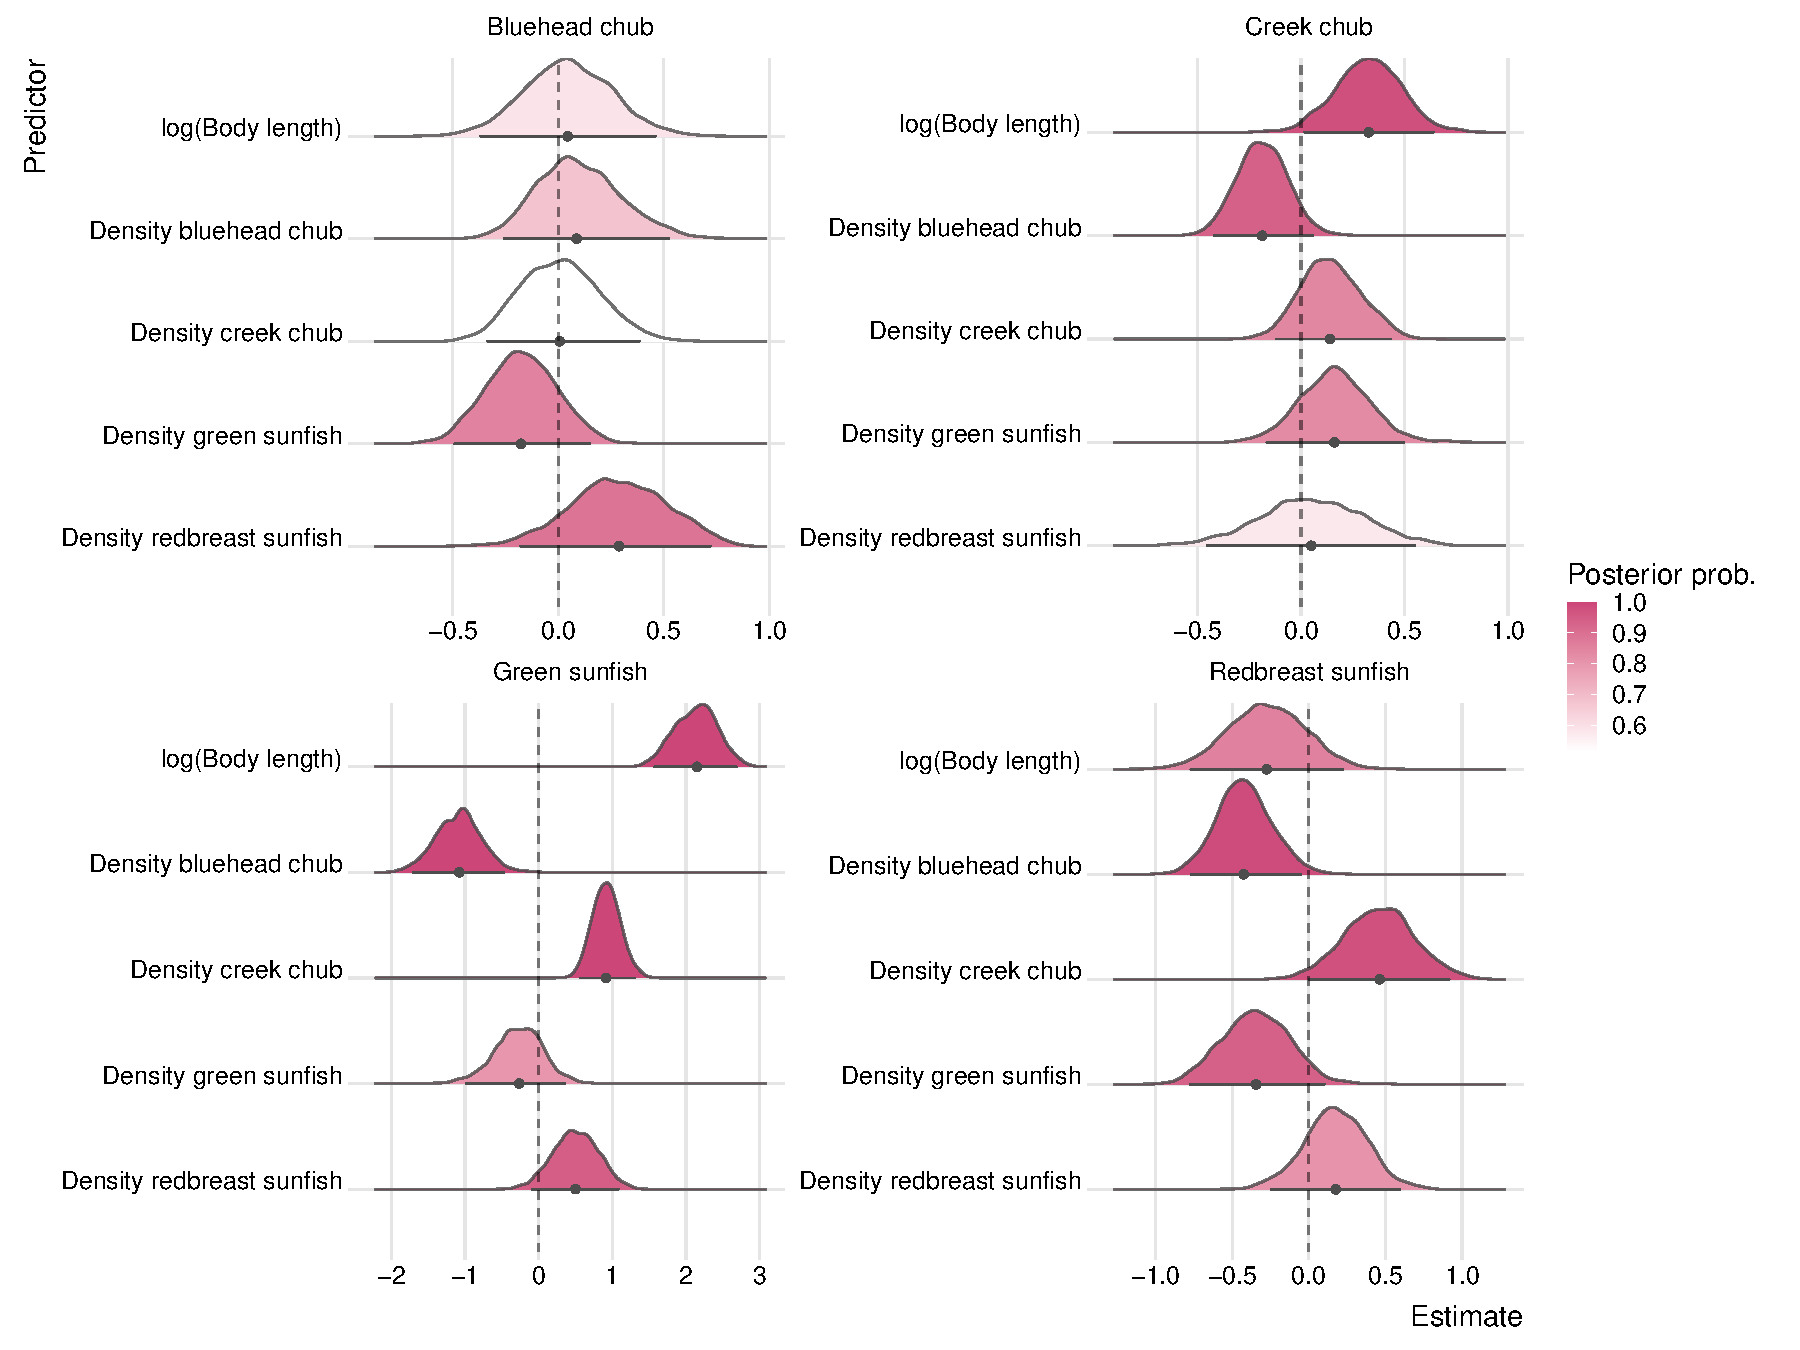
\includegraphics[width=0.8\linewidth]{output/fig_est.pdf}
    \caption{Parameter estimates from the dispersal-observation model. Median estimates are denoted by points with error bars showing the 95\% credible interval. Colors differentiate between significance with gray error bars showing insignificance, while blue lines are significant results.}
    \label{fig:fig_est}
\end{figure}
Our model revealed that movement based on length and density is species-specific with similar trends exhibited at the family-level (Figure \ref{fig:fig_est}). In cyprinid species, both species tended to increase movement distance with their body size, although the effect was insignificant for bluehead chub (Figure \ref{fig:fig_size}). Body size had contrasting influences on centrachid species, with larger individuals moving more in green sunfish (Figure \ref{fig:fig_size}). However, the effect of size on redbreast sunfish was insignificant.
\begin{figure}
    \centering
    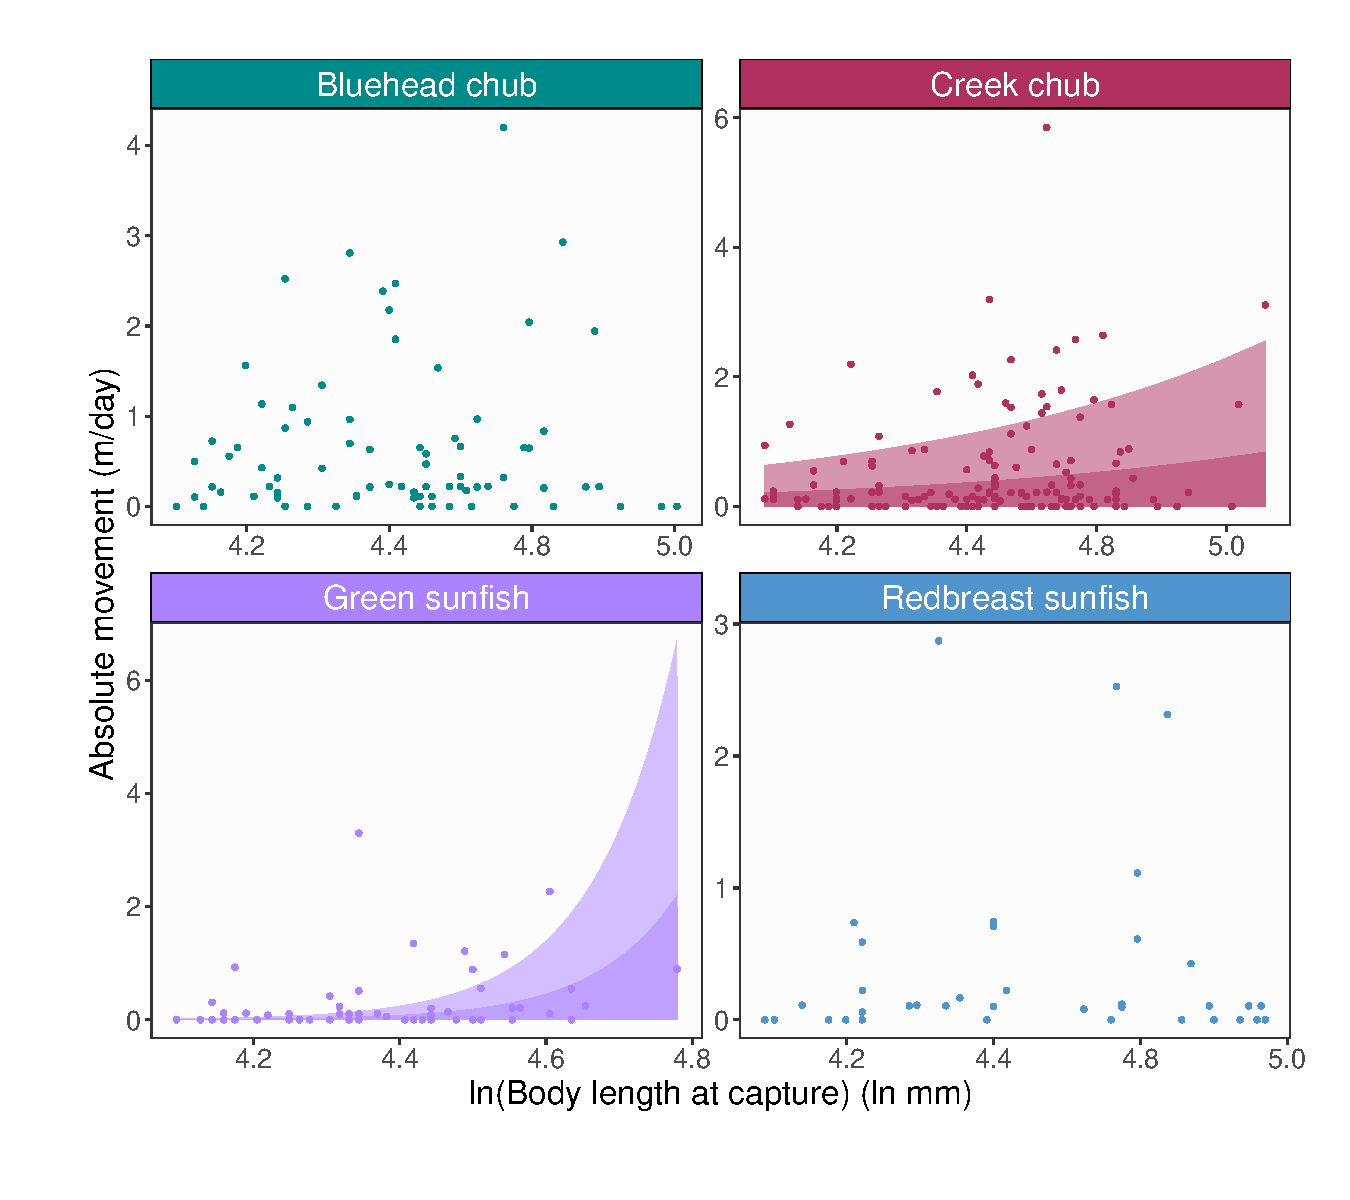
\includegraphics[width=0.75\linewidth]{output/fig_size.pdf}
    \caption{Response of body size on movement distance. Panels and colors show absolute movement per day of each species in response to an individual's total length at capture. Points represent actual values for each recaptured individual. Lines indicate the modeled movement estimate in response to length (significant = solid, insignificant = dashed).}
    \label{fig:fig_size}
\end{figure}
Cyprinid species (creek chub and bluehead chub) responded vaguely to population densities. Two exceptions exist: the negative effect of redbreast sunfish on creek chub, and the positive effect of bluehead chub on bluehead chub (Figure \ref{fig:fig_density}). The bluehead chub species was the only one to respond significantly to their conspecific densities. Centrarchid species responded more clearly to population densities. Green sunfish responded to high densities of redbreast sunfish by reducing movements. Both species increased their movements as the density of creek chub increases, while decreasing movements in areas with a high density of bluehead chub (Figure \ref{fig:fig_density}).

\begin{figure}
    \centering
    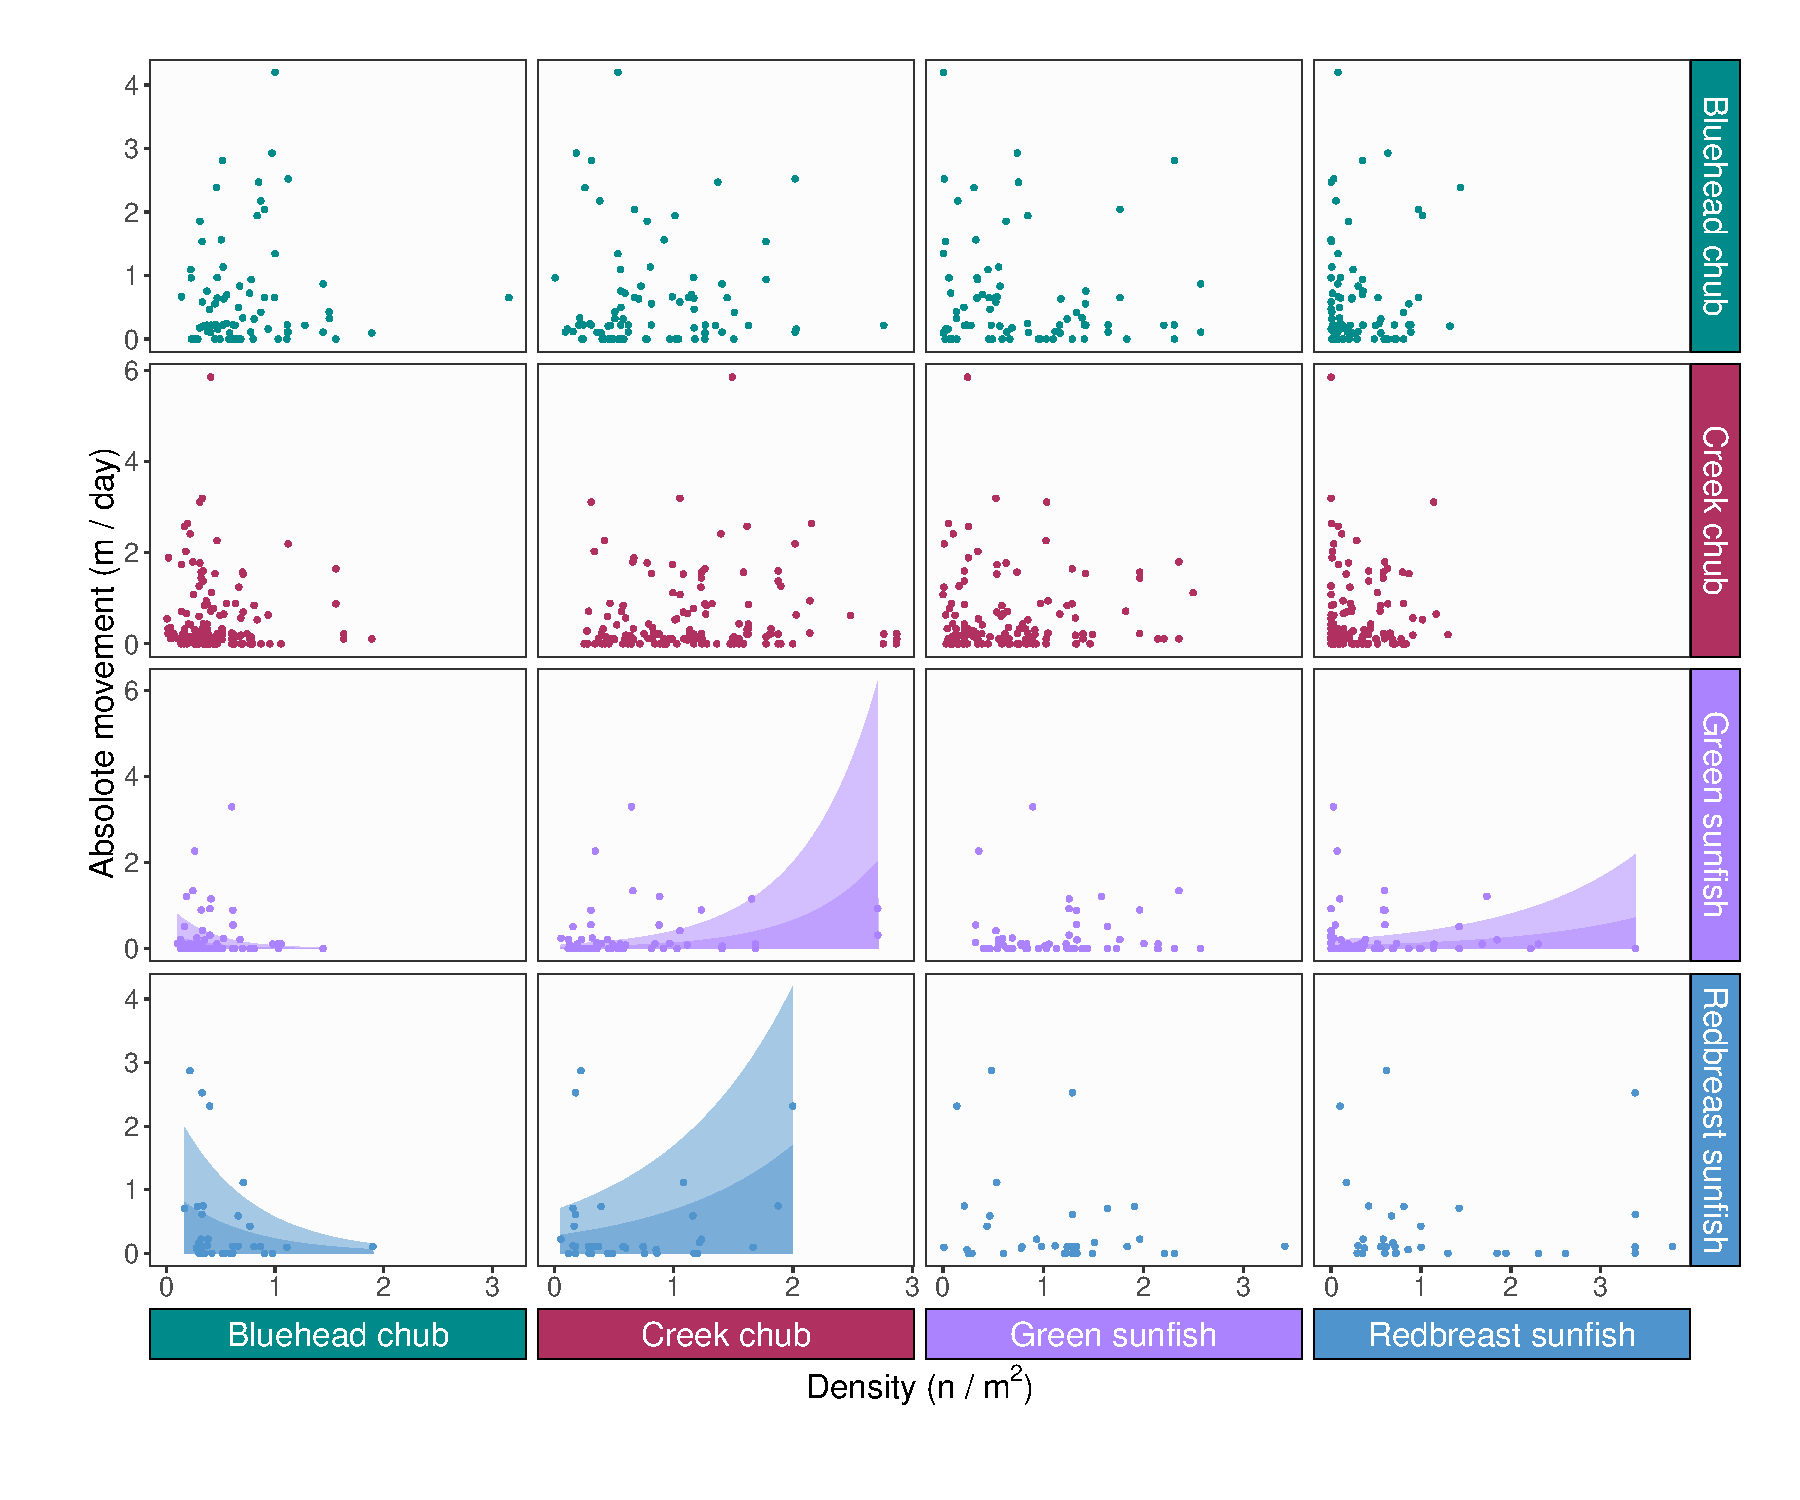
\includegraphics[width=0.8\linewidth]{output/fig_density.pdf}
    \caption{Response of density on movement distance. Each panel describes the absolute movement of a species (rows) in response to the density of a given species (column). Colors represent species. Diagonally, the response to intraspecific interactions are shown, while anything outside the diagonal is the response to interspecific interactions. Points represent actual values for each recaptured individual. Lines indicate the modeled movement estimate in response to density (significant = solid, insignificant = dashed).}
    \label{fig:fig_density}
\end{figure}

Both centrarchid species responded to undercut bank areas. Green sunfish movements increased as HRA increased, while redbreast sunfish movements declined. Neither cyprinid species was impacted by HRA. Temperature was only significant for bluehead chub by minimizing movements as temperature increased. Velocity had a negative effect on all four species except for bluehead chub, driving less movement as velocity increases. 

\section{Discussion}

Movement is shaped by species responses to extrinsic and intrinsic drivers \citep{clobertDispersalEcologyEvolution2012}. Yet, these factors are often studied in isolation, causing a lack of quantitative analysis comparing their relative influences. Our four-year data set of mark-recapture research unveiled that both extrinsic (population densities) and intrinsic (body size) factors influence stream fish movements, but their influences varied among families. Centrarchids (green sunfish and redbreast sunfish) react more clearly to the extrinsic variable, while weak patterns persist among cyprinids. Conversely, cyprinids behave akin to one another in response to the intrinsic variable, whereas centrarchids show diverging responses. While these movement patterns seem complicated, understanding species-level movement responses can provide greater insight into how species interactions are distributed by non-random movement. 

Our results partially supported our first prediction that higher interspecific density drivers more movement. Centrarchid species (green sunfish and redbreast sunfish) moved longer distances as the density of creek chub increased. This positive interspecific density-dependence may be indicative of competition between species and in response, certain competitors (sunfish species in this case) may favor moving to potentially suboptimal habitats in order to avoid this type of interaction \citep{jacobHabitatChoiceMeets2018, thierryInterplayAbioticBiotic2024}. Sunfish, particularly the green sunfish, may be successful in this approach as they are a hardy species that colonizes new areas well \citep{lemlySuppressionNativeFish1985, moyleInlandFishesCalifornia2002}. In small streams, the diets of both cyprinids and centrarchids overlap significantly \citep{collarPISCIVORYLIMITSDIVERSIFICATION2009, lemlySuppressionNativeFish1985, karrAssessmentBioticIntegrity1981, leonardApplicationTestingIndex1986}, potentially explaining the mechanism behind this interpretation.  

Centrarchid species, however, responded contrastingly to high bluehead chub densities by exhibiting less movement. Predator-prey interactions may underlie this negative interspecific density-dependence \citep{jacobHabitatMatchingSpatial2015}. Redbreast sunfish have been found predating on various chub species \citep{borrelliPuttingLakeTogether2023}, so perhaps the bluehead chub acts as a potential prey species discouraging sunfish to move because of accessible food resources. Predation of bluehead chub has been documented to occur in green sunfish \citep{lemlySuppressionNativeFish1985}, making it probable in redbreast sunfish as well. Alternatively, shared environmental cues between the species, such as greater microhabitat (undercut bank, wood debris) availability, could explain a decrease in movement because these areas provide added refugia \citep{careyEffectsLittoralHabitat2010}. While we cannot rule out the possibility of shared environmental cues, this mechanism is unlikely because the effects of microhabitat availability were statistically controlled in our model. Although experimental approaches are needed to elucidate biological causality, the trophic mechanism is more likely in our study system. 

Cyprinid species (bluehead chub and creek chub) showed unclear responses to interspecific population density. The only exception was the decreased movement of creek chub in areas with higher redbreast sunfish density. Similar to the story above, predator-prey interactions may explain this observed pattern. Creek chubs are known omnivores feeding on a variety of insects, detritus, and fish \citep{champagneRiparianBuffersMaintain2022, leonardApplicationTestingIndex1986, quistSummerFoodHabits2006}. While there is no direct evidence for creek chubs predating upon redbreast sunfish, it is conceivable that larger creek chubs feed on smaller redbreast sunfish given the omnivorous nature of creek chubs.

Interestingly, only the bluehead chub responded significantly to intraspecific densities, countering our second prediction. This result is somewhat surprising given the wealth of studies showing intraspecific competition exceeding interspecific competition in fishes \citep{websterMechanismsIndividualConsequences2000, wardIntraspecificFoodCompetition2006} and other taxa \citep{adlerCompetitionCoexistencePlant2018, barabasEffectIntraInterspecific2016, thompsonProcessbasedMetacommunityFramework2020, chessonRolesHarshFluctuating1997, tilmanResourceCompetitionCommunity1982, mcpeekIntraspecificDensityDependence2012}. While high conspecific density could impose intensive intraspecific competition, it also increases the likelihood of finding potential mates, dilution effects, and group feeding (e.g., Allee effects)\citep{courchampAlleeEffectsEcology2008, gascoigneAlleeEffectsDriven2004, teruiCrypticAlleeEffect2015}. In our system, this may overshadow the relative competition for other resources like habitat and food, thus producing stronger interspecific competition. This effect can be exacerbated when body size is considered because larger individuals can impose stronger interspecific competition on smaller individuals that utilize the same resource. Although further studies are needed to illuminate underlying mechanisms, these opposing influences of conspecific density could potentially obscure the influence on movement patterns. 

Our third prediction, the positive influence of body size on movement, was partially supported (creek chub and green sunfish). Movement requires great energetic expenditure that needs to be balanced among an individual’s needs \citep{boisclairImportanceActivityBioenergetics1989, joblingBioenergeticsFeedIntake1993, cookeMovementEcologyFishes2022}. Body size is one such limiting factor in determining metabolism \citep{beamish2SwimmingCapacity1978, rubio-graciaSizerelatedEffectsInfluence2020}. Because larger individuals have lower relative maintenance costs than smaller individuals due to greater lipid reserves \citep{brownSizeMattersTest2004, krauseRefugeUseFish1998, kannoBodyConditionMetrics2023}, they may be better able to balance the cost of moving \citep{schlagelMovementmediatedCommunityAssembly2020}. Not only are larger individuals at an energetic advantage, but they may serve as a stronger competitor in the settlement phase \citep{rasmussenIndividualMovementStream2017}. This mechanism, in conjunction with our result that high densities of creek chubs drive sunfish movement, may further support the idea that sunfish are adept to successful colonization when faced with competitive interactions. While this may also explain, in part, the positive relationship between movement and body size in green sunfish, we cannot rule out the possibility of statistical artifacts arising from the low recaptures of larger-bodied green sunfish. 

Movement is complex and nature cannot always follow a clear pattern as exemplified by our results. While we selected an extrinsic and intrinsic variable representative of species interactions and individual movement ability, other potential variables may be playing a role in driving movement (e.g., sex, disturbance) that we were unable to quantify. Additionally, we experienced relatively low consecutive recapture rates, likely because of the small spatial extent of our study area. Our dispersal-observation model accounted for emigration, imperfect detection, and survival processes to minimize statistical biases arising from this limitation. Yet, it is not possible to completely eliminate the limitation of our mark-recapture approach. Future studies addressing these limitations could provide deeper insight into the ecological drivers of movement.

Movement mediates how species interact shaping communities and metacommunities \citep{schlagelMovementmediatedCommunityAssembly2020}. Our study demonstrates how intrinsic (e.g., body size) and extrinsic (e.g., population density) drivers can help pinpoint potential movement patterns in freshwater fishes with variation among species elucidating a potential avenue to explore community dynamics in the future. Extrapolating how non-random movements, such as those identified in this study, affect species coexistence and the spatial patterns of community organization will be essential in connecting behavioral ecology to spatial theory. Although metapopulation and metacommunity, two major frameworks in spatial ecology, typically assume movement or dispersal processes are stochastic, recent theoretical studies have begun to incorporate non-random movement into their simulation frameworks \citep{amarasekareEffectNonrandomDispersal2010, ruokolainenStableCoexistenceEcologically2016}. Yet, empirical validations lag far behind. Integrating field-based movement patterns with theoretical simulations will provide greater insight into the mechanisms behind community and metacommunity dynamics.


\bibliography{tex/references}

\end{document}